% ======================================================================================================
% TCC - César Henrique Bernabé
% Capítulo 2 - Referencial Teórico
% Falar sobre os problemas do modelo antigo do zanshin
% Falar sobre novo metamodelo e explicar como cheguei nele
% Falar o prq do novo metamodelo ser melhor que o anterior e quais as novidades
% Falar sobre as vantagens do novo metamodelo no arquivo XML
% Falar das restricoes inseridas no novo metamodelo
% Falar dos problemas do novo metamodelo
% Falar de refinamentos (OR, AND, só pode ser AND ou OR, etc) e que agora quase todos os requisitos possuem refinamentos
% 
% ======================================================================================================
\chapter{Referencial Teórico}
\label{sec-referencial}

Este capítulo apresenta os principais conceitos teóricos que fundamentaram a evolução do metamodelo de requisitos do \zanshin e do desenvolvimento da ferramenta \unagi. A seção~\ref{sec-referencial-engenharia-requisitos} aborda a Engenharia de Requisitos Orientada a Objetivos, destacando os principais conceitos dessa área que foram utilizados ao longo deste trabalho. A seção~\ref{sec-referencial-zanshin} apresenta o sistema \zanshin e os detalhes do metamodelo original do \textit{framework}. A seção~\ref{sec-referencial-unagi} apresenta as principais ferramentas que foram utilizadas durante o desenvolvimento do \unagi, como as funcionalidades de Desenvolvimento Orientado a Modelos (\textit{Model Driven Development} ou MDD) do \eclipse, o plugin \sirius, dentre outros.

% ======================================================================================================
% SEÇÃO Engenharia de Requisitos Orientada a Objetivos
% ======================================================================================================

\section{Engenharia de Requisitos Orientada a Objetivos}
\label{sec-referencial-engenharia-requisitos}

A \textbf{Engenharia de Requisitos Orientada a Objetivos} é uma parte subárea de Engenharia de Requisitos, componente da área de Engenharia de Software. 

%TODO: Falar brevemente sobre engenharia de software, engenharia de requisitos e então engenharia de objetivos.

Objetivos são parte importante do processo Engenharia de Requisitos, seu propósito é indicar as principais necessidades que levaram a criação de um determinado sistema, demonstrando os casos em que as funcionalidades do mesmo satisfarão as necessidades elicitadas, além de dizer como o sistema deve ser construído para satisfazê-las ~\cite{ross1977structured}. Em uma descrição geral e resumida do processo de identificação de objetivos, pode-se dizer que o potencial software é analisado nos ambientes organizacional, operacional e técnico, onde são assim identificados os problemas do contexto e as oportunidades de solução desses problemas com o desenvolvimento do sistema. Então, os objetivos são criados com foco na resolução dos problemas e das oportunidades identificadas. Tendo em mãos os objetivos do sistema devidamente refinados e elaborados, os requisitos do sistema são então elaborados para que esses objetivos sejam devidamente atendidos. Além de apoiar no processo de modelagem de requisitos, objetivos são usados para apoiar outros propósitos como gerenciamento de conflitos e verificação ~\cite{van2001goal}. De acordo com ~\cite{van2001goal}, ~\cite{jackson1995software} e ~\cite{zave1997four}, objetivos podem ser reformulados de em diferentes níveis de abstração, dependendo do tipo de necessidade que o sistema alvo deve atender, abrangendo desde interesses referentes a estratégias de negócios até conceitos técnicos de atividades, podendo assim refererir-se a requisitos funcionais e não-funcionais.

A necessidade de uso de objetivos no processo de modelagem de sistemas de softwares vem se tornando cada vez mais clara, a medida que analistas percebem que a Engenharia de Objetivos é importante pois:
\begin{itemize}
	\item Objetivos provêm critérios claros de completude dos requisitos do sistema, permitindo também que requisitos desnecessários sejam descartados.
	\item Facilita o processo de entendimento dos requisitos por parte dos \textit{stakeholders}.
	\item Melhora a legibilidade de documentos de especificação de requisitos, pois permite que engenheiros possam enxergar com mais clareza as alternativas de desenvolvimento requisitos do sistema. Além de facilitar o processo de gerenciamento de conflitos.
	\item Objetivos dirigem parte do processo de elicitação de requisitos, facilitando a identificação de boa parte deles.
	
\end{itemize}

Diferentemente dos requisitos, objetivos podem precisar da cooperação entre diferentes agentes para que sejam atendidos de forma suficiente ~\cite{dardenne1993goal}. Em outras palavras, um objetivo sob responsabilidade de um agente único dentro sistema a ser criado torna-se um requisito, enquanto um objetivo sob responsabilidade de um agente dentro ambiente em que o software será executado torna-se uma Pressuposição de Domínio e nesse caso são satisfeitos devido a uma regra de negócio ~\cite{van2001goal, van1998managing}. Da mesma forma, objetivos podem ser classificados como objetivos rígidos (\textit{Hard Goals}) e objetivos fracos (\textit{Soft Goals}), estes não possuem critérios claros de satisfação, entretanto são úteis quando deseja-se comparar os melhores refinamentos ao objetivo estudado, enquanto aqueles são objetivos cujo critério de satisfação pode ser atendido de forma técnica ~\cite{dardenne1993goal}.




% ======================================================================================================
% SUBSEÇÃO Análise e Especificação de Requisitos
% ======================================================================================================

\subsection{Análise e Especificação de Requisitos}
\label{sec-referencial-engenharia-software-atividade-desenvolvimento-analise-especificacao-requisisto}

O foco está no levantamento, compreensão e especificação dos requisitos que o sistema a ser desenvolvido tem de tratar.  Erros nesta fase são mais dificéis de serem corrigidos quando identificados posteriormente, assim é importante entender o que o cliente deseja.% i

No que concerne às atividades técnicas, tipicamente o processo de software inicia-se com o Levantamento de Requisitos, quando os requisitos do sistema a ser desenvolvido são preliminarmente capturados e organizados. Uma vez capturados, os requisitos devem ser modelados, avaliados e documentados. Uma parte essencial dessa fase é a elaboração de modelos descrevendo o que o software tem de fazer (e não como fazê-lo), dita Modelagem Conceitual. Até este momento, a ênfase está sobre o domínio do problema e não se deve pensar na solução técnica, computacional a ser adotada~\cite{falboEngReq}.

Dada a importância dos requisitos para o sucesso de um projeto, atividades de controle da qualidade devem ser realizadas para verificar, validar e garantir a qualidade dos requisitos, uma vez que os custos serão bem maiores se defeitos em requisitos forem identificados tardiamente~\cite{falboEngReq}.

Neste projeto foram utilizadas as técnicas de levantamento e especificação de requisitos aprendidas ao longo do curso, como descrição de minimundo, levantamento de requisitos funcionais e não-funcionais, modelagem de casos de uso e modelagem conceitual estrutural. Nos parágrafos que se seguem, descrevemos brevemente estas técnicas.

A descrição do minimundo apresenta, em um texto corrido, uma visão geral do domínio do problema a ser resolvido e dos processos de negócio apoiados, bem como as principais ideias do cliente sobre o sistema a ser desenvolvido.

Já os requisitos funcionais, são declarações de serviços que o sistema deve prover, descrevendo o que o sistema deve fazer, podendo descrever, ainda, como o sistema deve reagir a entradas específicas, como o sistema deve se comportar em situações específicas e o que o sistema não deve fazer~\cite{sommerville}.

Assim como os requisitos funcionais precisam ser especificados em detalhes, o mesmo acontece com os requisitos não-funcionais. Para os atributos de qualidade considerados prioritários, o analista deve trabalhar no sentido de especificá-los de modo que eles se tornem mensuráveis e, por conseguinte, testáveis. Eles descrevem restrições sobre os serviços ou funções oferecidos pelo sistema~\cite{sommerville}.

O modelo de casos de uso é um modelo comportamental, mostrando as funções do sistema, mas de maneira estática. Ele é composto de dois tipos principais de artefatos: os diagramas de casos de uso e as descrições de casos de uso. Um diagrama de casos de uso é um diagrama bastante simples, que descreve o sistema, seu ambiente e como sistema e ambiente estão relacionados. As descrições dos casos de uso descrevem o passo a passo para a realização dos casos de uso e são essencialmente textuais~\cite{falboEngReq}. 

Tomando por base casos de uso e suas descrições, é possível passar à modelagem conceitual estrutural, quando os conceitos e relacionamentos envolvidos no domínio são capturados em um conjunto de diagramas de classes. Neste momento é importante definir, também, o significado dos conceitos e de suas propriedades, bem como restrições sobre eles. Essas definições são documentadas em um dicionário de dados do projeto.

Um diagrama de classes exibe um conjunto de classes e seus relacionamentos. Diagramas de classes proveem uma visão estática da estrutura de um sistema e, portanto, são usados na modelagem conceitual estrutural. Para tornar os modelos conceituais mais simples, de modo a facilitar a comunicação com clientes e usuários, tipos de dados de atributos podem ser omitidos do diagrama de classes. Restrições de integridade são regras de negócio e poderiam ser lançadas no Documento de Requisitos. Contudo, como elas são importantes para a compreensão e eliminação de ambiguidades do modelo conceitual, é útil descrevê-las no próprio modelo conceitual~\cite{falboEngReq}. 




% ======================================================================================================
% SUBSEÇÃO Projeto
% ======================================================================================================

\subsection{Projeto}
\label{sec-referencial-engenharia-software-atividade-desenvolvimento-projeto}

Com os requisitos pelo menos parcialmente capturados e especificados na forma de modelos, pode-se começar a trabalhar no domínio da solução. Muitas soluções são possíveis para o mesmo conjunto de requisitos e elas são intrinsecamente ligadas a uma dada plataforma de implementação (linguagem de programação, mecanismo de persistência a ser adotado etc.). A fase de projeto tem por objetivo definir e especificar uma solução a ser implementada. É uma fase de tomada de decisão, tendo em vista que muitas soluções são possíveis~\cite{falboEngReq}.

A fase de Projeto é responsável por incorporar requisitos tecnológicos aos requisitos essenciais do sistema e, portanto, requer que a plataforma de implementação seja conhecida. Basicamente, envolve duas grandes etapas: projeto da arquitetura do sistema e o projeto detalhado. O objetivo da primeira etapa é definir a arquitetura geral do software, tendo por base o modelo construído na fase de análise de requisitos. Essa arquitetura deve descrever a estrutura de nível mais alto da aplicação e identificar seus principais componentes. O propósito do projeto detalhado é detalhar o projeto do software para cada componente identificado na etapa anterior. Os componentes de software devem ser sucessivamente refinados em níveis maiores de detalhamento, até que possam ser codificados e testados~\cite{falboEngSoft}. 





% ======================================================================================================
% SEÇÃO FrameWeb
% ======================================================================================================

\section{FrameWeb}
\label{sec-referencial-frameweb}

FrameWeb (\textit{Framework-based Design Method for Web Engineering}) é um método de projeto para construção de sistemas de informação Web (\textit{Web Information Systems – WISs}) baseados em \textit{frameworks}. FrameWeb é baseado em metodologias e linguagens de modelagem bastante difundidas na área de Engenharia de Software sem, no entanto, impor nenhum processo de desenvolvimento específico~\cite{vitorFrameWeb}.

A proposta deste método foi motivada por:

\begin{itemize}
	\item O uso de \textit{frameworks} ou arquiteturas baseadas em \textit{containers} similares a eles se tornou o padrão de fato para o desenvolvimento de aplicações distribuídas, em especial os baseados na plataforma Web;
	
	\item O uso de métodos que se adequam diretamente à arquitetura de software adotada promove uma agilidade maior ao processo, característica que é bastante desejada na maioria dos projetos Web~\cite{presmannSoft}.
\end{itemize}

Em linhas gerais, FrameWeb assume que determinados tipos de \textit{frameworks} serão utilizados durante a construção da aplicação, define uma arquitetura básica para o WIS e propõe modelos de projeto que se aproximam da implementação do sistema usando esses \textit{frameworks}.

Devido à popularidade dos \textit{frameworks} no desenvolvimento web, o método FrameWeb propõe a utilização de modelos específicos direcionados à arquitetura baseada em \textit{containers}, que durante a fase de projeto auxiliam o modelador na tarefa de lidar com a complexidade por trás da aplicação WIS. Porém, não só novos \textit{frameworks}, tecnologias e plataformas surgiram, como continuarão surgindo e evoluindo. Por isso, é importante que os métodos também evoluam não só no que diz respeito a novas versões, mas também para permitir que as novidades possam ser incorporadas de forma simples e efetiva, como propõe~\citeonline{martins-mestrado15}.

Sendo um método para a fase de projeto, não prescreve um processo de software completo. No entanto, sugere o uso de um processo de desenvolvimento que contemple as fases apresentadas na Figura~\ref{fig-referencial-processo-software}. Para uma melhor utilização de FrameWeb, espera-se que sejam construídos diagramas de casos de uso e de classes de domínio (ou similares) durante as fases de Requisitos e Análise. 

\begin{figure}[h]
	\centering
	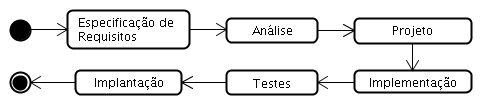
\includegraphics[width=1\textwidth]{figuras/referencial/fig-referencial-processo-software}
	\caption{Processo de Desenvolvimento de Software~\cite{vitorFrameWeb}.}
	\label{fig-referencial-processo-software}
\end{figure}

A fase de Projeto concentra as propostas principais do método: (i) definição de uma arquitetura padrão que divide o sistema em camadas, de modo a se integrar bem com os \textit{frameworks} utilizados; (ii) proposta de um conjunto de modelos de projeto que trazem conceitos utilizados pelos \textit{frameworks} para esta fase do processo por meio da criação de um perfil UML que faz com que os diagramas fiquem mais próximos da implementação.

O FrameWeb define extensões leves (\textit{lightweight extensions}) ao meta-modelo da UML para representar componentes típicos da plataforma Web e dos \textit{frameworks} utilizados, criando um perfil UML que é utilizado para a construção de diagramas de quatro tipos:

\begin{itemize}
	\item \textbf{Modelo de Domínio:} é um diagrama de classes da UML que representa os objetos de domínio do problema e seu mapeamento para a persistência em banco de dados relacional. Os passos para sua construção são:
	
	\begin{itemize}
		\item A partir do modelo de classes construído na fase de análise de requisitos, adequar o modelo à plataforma de implementação escolhida, indicando os tipos de dados de cada atributo, promovendo a classes atributos que devam ser promovidos, definindo a navegabilidade das associações etc.;
		\item Adicionar os mapeamentos de persistência.	
		
	\end{itemize}
	
	\item \textbf{Modelo de Aplicação:} é um diagrama de classes da UML que representa as classes de serviço, que são responsáveis pela codificação dos casos de uso, e suas dependências. Os passos para a construção do Modelo de Aplicação são:	
	\begin{itemize}
		\item Analisar os casos de uso modelados durante a Especificação de Requisitos, definir a granularidade das classes de serviço e criá-las. Utilizar, preferencialmente, nomes que as relacionem com os casos de uso ou cenários que representam;
		
		\item Adicionar às classes/interfaces os métodos que implementam a lógica de negócio, com atenção ao nome escolhido (preferencialmente relacionar o método ao cenário que implementa), aos parâmetros de entrada e ao retorno (observar a descrição do caso de uso);
		
		\item Por meio de uma leitura da descrição dos casos de uso, identificar quais DAOs (\textit{Data Access Object})~\cite{alurDAO} são necessários para cada classe de aplicação e modelar as associações;
		
		\item Voltar ao modelo de navegação (se já foi construído), identificar quais classes controladoras dependem de quais classes de serviço e modelar as associações.
	\end{itemize}
	
	\item \textbf{Modelo de Navegação:} é um diagrama de classe da UML que representa os diferentes componentes que formam a camada de Lógica de Apresentação, como páginas Web, formulários HTML e classes controladoras. Os passos para a construção dos Modelos de Navegação são:
	\begin{itemize}
		\item Analisar os casos de uso modelados durante a Especificação de Requisitos, definir a granularidade das classes controladoras e criá-las, definindo seus métodos. Utilizar, preferencialmente, nomes que as relacionem com os casos de uso ou cenários que representam;
		\item Identificar como os dados serão submetidos pelos clientes para criar as páginas, modelos e formulários, adicionando atributos à classe controladora;
		\item Identificar quais resultados são possíveis a partir dos dados de entrada, para criar as páginas e modelos de resultado, também adicionando atributos à classe controladora.
		\item Analisar se o modelo ficou muito complexo e considerar dividi-lo em dois ou mais diagramas.
	\end{itemize}
	
	\item \textbf{Modelo de Persistência:} é um diagrama de classes da UML que representa as classes DAO existentes, responsáveis pela 	persistência das instâncias das classes de domínio. Os passos para a construção desse modelo são:
	\begin{itemize}
		\item Criar as interfaces e implementações concretas dos DAOs base;
		\item Definir quais classes de domínio precisam de lógica de acesso a dados e, portanto, precisam de um DAO;	
		\item Para cada classe que precisa de um DAO, avaliar a necessidade de consultas específicas ao banco de dados, adicionando-as como operações nos respectivos DAOs.
	\end{itemize}
	O Modelo de Persistência apresenta, para cada classe de domínio que necessita de lógica de acesso a dados, uma interface e uma classe concreta DAO que implementa a interface. A interface, que é única, define os métodos de persistência existentes para aquela classe, a serem implementados por uma ou mais classes concretas, uma para cada tecnologia de persistência diferente (ex.: um DAO para o JPA, outro para o \textit{framework} OJB, etc.).
	
\end{itemize}

Esses quatro modelos serão descritos na Seção~\ref{sec-projeto-modelos-frame-web} no contexto do SAE, sistema desenvolvido neste trabalho.






% ======================================================================================================
% SEÇÃO Desenvolvimento Web
% ======================================================================================================

\section{Desenvolvimento Web}
\label{sec-referencial-desenvolvimento-web}

As aplicações Web de hoje em dia já possuem regras de negócio bastante complicadas. Codificar essas regras já representa um grande trabalho. Além dessas regras, conhecidas como requisitos funcionais de uma aplicação, existem outros requisitos (não-funcionais) que precisam ser atingidos através da infraestrutura do sistema: persistência em banco de dados, transação, acesso remoto, \textit{web services}, gerenciamento de \textit{threads}, gerenciamento de conexões HTTP, \textit{cache} de objetos, gerenciamento da sessão web, balanceamento de carga, entre outros~\cite{caelumDesenvolvimento}.

A Java EE (\textit{Java Platform, Enterprise Edition}) é uma plataforma padrão para desenvolver aplicações Java de grande porte e/ou para a Internet, que inclui bibliotecas e funcionalidades para implementar software Java distribuído, baseado em componentes modulares que executam em servidores de aplicações e que suportam escalabilidade, segurança, integridade e outros requisitos de aplicações corporativas ou de grande porte~\cite{thiagoJava}.

A plataforma Java EE possui uma série de especificações (tecnologias) com objetivos distintos, por isso é considerada uma plataforma guarda-chuva. Entre as especificações da Java EE, as mais conhecidas são:

\begin{itemize}
	\item \textbf{Servlets}: são componentes Java executados no servidor para gerar conteúdo dinâmico para a web, como HTML e XML.
	\item \textbf{JSF (\textit{JavaServer Faces})}: é um framework web baseado em Java que tem como objetivo simplificar o desenvolvimento de interfaces de sistemas para a web, através de um modelo de componentes reutilizáveis. 
	\item \textbf{JPA (\textit{Java Persistence API})}: é uma API padrão do Java para persistência de dados, baseada no conceito de mapeamento objeto-relacional. Essa tecnologia traz alta produtividade para o desenvolvimento de sistemas que necessitam de integração com banco de dados. 
	\item \textbf{EJB (\textit{Enterprise Java Beans})}: são componentes que executam em servidores de aplicação e possuem como principais objetivos fornecer facilidade e produtividade no desenvolvimento de componentes distribuídos, transacionados, seguros e portáveis.
	\item \textbf{JAAS (\textit{Java Autenthication and Authorization Service})}: API padrão do Java para segurança.
	\item \textbf{CDI (\textit{Contexts and Dependency Injection})}: é a especificação da Java EE que trabalha com injeção de dependências.	
\end{itemize}





% ======================================================================================================
% SUBSEÇÃO Servlets
% ======================================================================================================

\subsection{\textit{Servlets}}

O nome \textit{servlet} vem da ideia de um pequeno servidor (servidorzinho, em inglês) cujo objetivo é receber chamadas HTTP, processá-las e devolver uma resposta ao cliente\cite{caelumDesenvolvimento}.

Uma primeira ideia da \textit{servlet} seria que cada uma delas é responsável por uma página, sendo que ela lê dados da requisição do cliente e responde com outros dados (uma página HTML, uma imagem GIF etc).

No mundo Java, os servidores web são chamados de \textit{Servlet Container}, pois implementam a especificação de \textit{Servlet}. O servidor converte a requisição em um objeto do tipo \textit{HttpServletRequest} . Este objeto é então passado aos componentes web, que podem executar qualquer código Java para que possa ser gerado um conteúdo dinâmico. Em seguida, o componente web devolve um objeto \textit{HttpServletResponse} , que representa a resposta ao cliente. Este objeto é utilizado para que o conteúdo gerado seja enviado ao navegador do usuário~\cite{thiagoJava}.






% ======================================================================================================
% SUBSEÇÃO EJB
% ======================================================================================================

\subsection{EJB}

EJBs simplificam o desenvolvimento de aplicações grandes e distribuídas. Primeiro, porque o \textit{container} EJB fornece serviços de nível de sistema a elas. Assim sendo o desenvolvedor pode se concentrar em resolver problemas do negócio. O \textit{container} EJB é responsável por serviços como gestão de transações e autorizações de segurança. Segundo, porque são os EJBs que contêm a lógica de negócios, não os clientes. Assim sendo, o desenvolvedor da aplicação cliente pode se concentrar na apresentação, não tendo que implementar regras de negócio ou bancos de dados de acesso. Como resultado, clientes tornam-se mais leves, executáveis em máquinas menos poderosas. Terceiro, porque EJBs são componentes portáteis, podendo ser reutilizados em outros aplicativos~\cite{PasteurEJB}. 

\textbf{\textit{Session Beans}} encapsulam lógica de negócio que pode ser invocada programaticamente por um cliente de maneira local, remota ou via web service. Para acessar uma aplicação armazenada em um servidor, o cliente invoca os métodos do \textit{Session Bean}. Sobre este tipo de EJB, trazemos as seguintes informações:

\textit{Stateful Session Beans:} em um EJB \textit{stateful}, suas variáveis de instância representam o estado de uma sessão única aberta entre o cliente e o EJB. Devido ao fato do cliente interagir com o EJB, esse estado é frequentemente denominado estado conversacional. O estado é mantido enquanto durar a sessão cliente/EJB.

\textit{Stateless Session Beans:} esses EJBs não mantêm um estado conversacional com o cliente. Quando o cliente invoca métodos de um EJB \textit{stateless}, as variáveis de instância mantêm um estado específico apenas enquanto durar a execução do método. Quando esta termina, o estado não é mantido. Exceto durante a invocação de métodos, todas as instâncias de EJBs \textit{stateless} são equivalentes, permitindo alocar uma instância para qualquer cliente. 

\textit{Singleton Session Beans:} são instanciados apenas uma vez por aplicação e existem durante o ciclo de vida da mesma. São projetados para circunstâncias nas quais uma única instância do EJB é compartilhada e concorrentemente acessada por clientes. Oferecem a mesma funcionalidade dos EJBs \textit{stateful}, a menos da instância única. O estado é mantido entre invocações de clientes, mas não quando ocorrem quedas do servidor. 

\textit{Acesso local:} o cliente deve estar na mesma aplicação do EJB. Pode ser um componente web ou outro EJB. \texttt{@Local} deve ser colocado no cabeçalho da interface do EJB local.

\textit{Acesso remoto:} pode rodar em uma máquina e JVM diferentes. Pode ser um componente web, uma aplicação cliente ou outro EJB. \texttt{@Remote} deve ser colocado no cabeçalho da interface do EJB remote.

\textbf{\textit{Message-Driven Beans}} são EJBs que permitem a aplicações Java EE processar mensagens assincronamente. Agem de maneira semelhante a um \textit{listener} (monitor) de eventos, mas ao invés de eventos, recebe mensagens provenientes de aplicações, outro EJB ou componentes web. Eles são acessados através de um serviço de mensagens (JMS), enviando mensagens ao destinatário (\textit{MessageListener}). São executados mediante a recepção de uma mensagem vinda do cliente, assincronamente e \textit{stateless}. Quando a mensagem chega, o \textit{container} chama o método \texttt{\textit{onmessage}} do \textit{Message-Driven Bean}, que por sua vez chama métodos auxiliares para processá-la. Tudo isso ocorre em um contexto transacional. Eles não são acessados via interfaces, como \textit{Session Beans}, ou seja, possuem apenas uma classe \textit{bean}~\cite{PasteurEJB}. 




% ======================================================================================================
% SUBSEÇÃO JSF
% ======================================================================================================

\subsection{JSF}

\textit{JavaServer Faces}, também conhecido como JSF, é uma tecnologia para desenvolvimento web que utiliza um modelo de interfaces gráficas baseado em eventos. Esta tecnologia foi definida pelo JCP (\textit{Java Community Process})\footnote{JCP -- https://www.jcp.org/en/home/index}, o que a torna um padrão de desenvolvimento e facilita o trabalho dos fornecedores de ferramentas, ao criarem produtos que valorizem a produtividade no desenvolvimento de interfaces visuais~\cite{thiagoJava}.

JSF é baseado no padrão de projeto MVC (\textit{Model-View-Controller})\footnote{MVC -- https://pt.wikipedia.org/wiki/MVC}, o que torna o desenvolvimento de sistemas menos complicado. O padrão MVC separa o sistema em três responsabilidades (modelo, visão e controle), onde o modelo é responsável por representar os objetos de negócio, manter o estado da aplicação e fornecer ao controlador o acesso aos dados. A visualização é responsável pela interface do usuário: ela que define a forma como os dados são apresentados e encaminha as ações do usuário para o controlador. O controlador é responsável por ligar o modelo e a visualização, interpretando as solicitações do usuário, traduzindo para uma operação no modelo e retornando a visualização adequada à solicitação~\cite{thiagoJava}.

Em JSF, o controle é feito através de uma \textit{servlet} chamada \textit{Faces Servlet}, opcionalmente configurada por arquivos XML e delegando o controle de requisições específicas aos vários manipuladores de ações e observadores de eventos implementados no sistema. Em resumo, a \textit{Faces Servlet} recebe as requisições dos usuários na web, redireciona para o modelo e envia uma resposta.

O verdadeiro poder de \textit{JavaServer Faces} está em seu modelo de componentes de interface do usuário, que gera alta produtividade aos desenvolvedores, permitindo a construção de interfaces para web usando um conjunto de componentes pré-construídos, ao invés de criar interfaces inteiramente do zero.

Existem vários componentes JSF, desde os mais simples, como um \emph{Output Label}, que apresenta simplesmente um texto, ou um \emph{Data Table}, que representa dados tabulares de uma coleção que pode vir do banco de dados. A API de JSF suporta a extensão e criação de novos componentes, que podem fornecer funcionalidades adicionais. Atualmente, existem diversas organizações que trabalham na criação de componentes personalizados, como exemplo, podemos citar a Oracle (\textit{ADF Faces Rich Client})\footnote{ADF -- http://www.oracle.com/technetwork/developer-tools/adf/overview/index-092391.html}, IceSoft (\textit{IceFaces})\footnote{IceFaces -- http://www.icesoft.org/java/projects/ICEfaces/overview.jsf}, Red Hat (\textit{RichFaces})\footnote{RichFaces -- http://richfaces.jboss.org/}, Prime Technology (\textit{PrimeFaces})\footnote{PrimeFaces -- http://www.primefaces.org/}, etc.

A biblioteca de componentes JSF utilizada neste trabalho foi a PrimeFaces. Ela inclui diversos campos de entrada, botões, tabelas de dados, árvores, gráficos, diálogos, etc~\cite{thiagoJava}.




% ======================================================================================================
% SUBSEÇÃO JPA
% ======================================================================================================

\subsection{JPA}
\label{sec-referencial-desenvolvimento-web-JPA}

Mapeamento objeto relacional (\textit{object-relational mapping, ORM, O/RM ou O/R mapping}) é uma técnica de programação para conversão de dados entre banco de dados relacionais e linguagens de programação orientada a objetos~\cite{thiagoJava}.
Em banco de dados, entidades são representadas por tabelas, que possuem colunas que armazenam propriedades de diversos tipos. Uma tabela pode se associar com outras e criar relacionamentos diversos.
Em uma linguagem orientada a objetos, como Java, entidades são classes, e objetos dessas classes representam elementos que existem no mundo real~\cite{thiagoJava}.

A \textit{Java Persistence API} (JPA) é um \textit{framework} para persistência em Java, que oferece uma API de mapeamento objeto-relacional e soluções para integrar persistência com sistemas corporativos escaláveis~\cite{thiagoJava}. Entre as vantagens podemos citar:

\begin{itemize}
	\item Códigos de acesso a banco de dados com \textit{queries SQL} são custosos de se desenvolver. JPA elimina muito do trabalho e deixa você se concentrar na lógica de negócio. JPA trará uma produtividade imensa para você.
	\item A manutenabilidade de sistemas desenvolvidos com ORM é excelente, pois o mecanismo faz com que menos linhas de código sejam necessárias. Além de facilitar o entendimento, menos linhas de código deixam o sistema mais fácil de ser alterado.
	\item ORM abstrai sua aplicação do banco de dados e do dialeto SQL. Com JPA, você pode desenvolver um sistema usando um banco de dados e colocá-lo em produção usando diversos outros banco de dados, sem precisar alterar códigos-fontes para adequar sintaxe de queries que só funcionam em SGBDs de determinados fornecedores.
\end{itemize}

Dentro do JPA, a API de Critérios (\textit{Criteria API}) é baseada no esquema abstrato de entidades persistentes (metamodelos), as suas relações e objetos incorporados. Esta API opera neste esquema abstrato para permitir que desenvolvedores de encontrar, modificar e excluir entidades persistentes invocando operações da JPA. Os metamodelos funcionam em conjunto com a API para modelar classes persistentes da entidade para consultas~\cite{oracleJAAS}.

O padrão DAO~\cite{alurDAO} adiciona uma camada de abstração a mais, separando a lógica de acesso a dados da tecnologia de persistência de maneira que a camada de aplicação não conheça qual \textit{framework} ORM está sendo utilizado, permitindo que o mesmo seja trocado, se necessário. O uso deste padrão também facilita a execução de testes unitários na camada de aplicação. 
Numa aplicação que utilize a arquitetura MVC, todas as funcionalidades de bancos de dados, tais como obter as conexões, mapear objetos Java para tipos de dados SQL ou executar comandos SQL, devem ser feitas por classes DAO. 

A vantagem de usar objetos de acesso a dados é a separação simples e rigorosa entre duas partes importantes de uma aplicação que não devem e não podem conhecer quase que nada uma da outra, e que podem evoluir frequentemente e independentemente. Alterar a lógica de negócio pode esperar apenas a implementação de uma interface, enquanto que modificações na lógica de persistência não alteram a lógica de negócio, desde que a interface entre elas não seja modificada. 



% ======================================================================================================
% SUBSEÇÃO JAAS
% ======================================================================================================

\subsection{JAAS}

Aplicações Java EE consistem em componentes que podem conter ambos os recursos protegidos e desprotegidos. Muitas vezes, é necessário proteger os recursos para garantir que somente usuários autorizados tenham acesso. Autorização fornece acesso controlado a recursos protegidos~\cite{oracleJAAS}.

\textit{Java Authentication and Authorization Service} (JAAS) é um conjunto de APIs que permitem serviços para autenticar e aplicar controles de acesso sobre os usuários. JAAS é parte do núcleo da Java SE API e é uma tecnologia de base para mecanismos de segurança Java EE. Os conceitos principais desta API são:

\begin{itemize}
	\item Autenticação: os meios pelos quais entidades comunicantes, como cliente e servidor, provam um ao outro que estão agindo em nome de identidades específicas que são autorizados para o acesso. Isso garante que os usuários são quem eles dizem que são~\cite{oracleJAAS}.
	
	\item Autorização ou controle de acesso: os meios pelos quais as interações com os recursos são limitados a grupos de usuários ou programas com o objetivo de impor a integridade, confidencialidade, disponibilidade ou restrições. Isso garante que os usuários têm permissão para executar operações ou dados de acesso~\cite{oracleJAAS}.
\end{itemize}

Um \textit{Role} (Papel) é um nome abstrato para a permissão de acesso a um determinado conjunto de recursos em um aplicação. Em uma aplicação que utiliza JAAS, um usuário só terá acesso à um recurso protegido se ele possuir um \textit{role} que permita este acesso, assim um \textit{role} pode ser comparado a uma chave que pode abrir uma fechadura. 

Para definir os recursos que serão protegidos e o mecanismo de autenticação na aplicação pode utilizar-se de um descritor de implementação. Em tempo de execução, o servidor Java EE lê este descritor de implementação e age sobre o correspondente aplicativo, em conformidade com as informações estruturais para cada módulo ou componente.

Restrição de segurança é usada para definir os privilégios de acesso a uma coleção de recursos utilizando o seu mapeamento de URL~\cite{oracleJAAS}. Este mapeamento é feito através de uma lista de padrões de URL (a parte de uma URL após o nome do \textit{host} e a porta que deseja restringir) e de operações HTTP que descrevem um conjunto de recursos a serem protegidos. Também é preciso definir quais os usuários terão permissão de executar essas requisições protegidas e como os dados serão protegidos quando transportados entre um cliente e um servidor.

Quando um mecanismo de autenticação for especificado no descritor de implementação, o usuário deve ser autenticado antes que o acesso seja concedido a qualquer recurso limitado por uma restrição de segurança. Pode haver várias restrições de segurança que se aplicam a vários recursos, mas o mesmo método de autenticação será aplicado a todos os recursos limitados em um aplicativo~\cite{oracleJAAS}.

A plataforma Java EE suporta os seguintes mecanismos de autenticação: autenticação básica, autenticação baseada em formulário, autenticação \textit{digest}, autenticação do cliente e autenticação mútua.

A \textbf{autenticação baseada em formulário} permite ao desenvolvedor controlar a aparência das telas de autenticação de login e de erro que um navegador HTTP apresenta para o usuário final. Quando a autenticação baseada em formulário é especificada, ocorrem as seguintes ações conforme a Figura~\ref{fig-referencial-jaas-method-form}.

\begin{figure}[h]
	\centering
	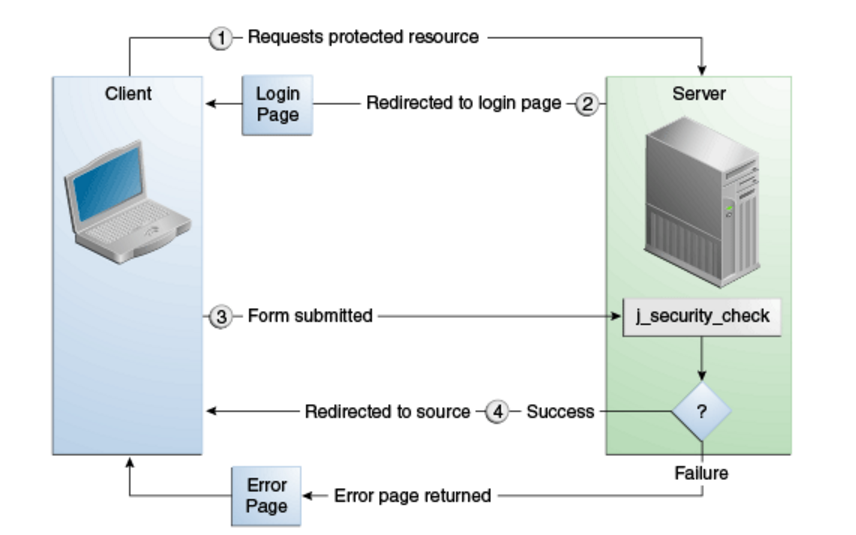
\includegraphics[width=1\textwidth]{figuras/referencial/fig-referencial-jaas-method-form}
	\caption{JAAS - Autenticação baseada em formulário~\cite{oracleJAAS}}
	\label{fig-referencial-jaas-method-form}
\end{figure}



Segurança declarativa permite o desenvolvedor de aplicações especificar quais usuários estão autorizados a acessar determinados métodos dos Enterprise Java Beans (EJBs). Um desenvolvedor que usa segurança declarativa para definir as permissões de métodos e mecanismos de autenticação passa junto ao implementador uma visão de segurança dos EJBs contidos em sua aplicação. Se você não definir uma visão da segurança, o implementador terá que determinar o que cada método de negócio faz para determinar quais usuários estão autorizados a chamar cada método.

A visão da segurança consiste de um conjunto de papéis de segurança, um agrupamento semântico de permissões que um determinado tipo de usuários de uma aplicação deve ter para acessá-lá com êxito. 

Permissões podem ser especificadas na classe, nos métodos da classe ou ambos. Permissões podem ser especificadas em um método da classe para substituir o valor das permissões especificado em toda a classe. As seguintes anotações são usadas para especificar permissões:

\begin{itemize}
	\item \texttt{@DeclareRoles}: especifica todas as roles que a aplicação irá utilizar, incluindo roles não designadas especificamente na uma anotação de \texttt{@RolesAllowed}.
	
	\item \texttt{@RolesAllowed}: especifica as roles de segurança autorizadas a métodos de acesso em um aplicação. Esta anotação pode ser especificada numa classe ou em um ou mais métodos. Quando especificada no nível de classe, a anotação aplica-se a todos os métodos na classe. Quando especificada em um método, a anotação aplica-se apenas ao método e substitui quaisquer valores especificados no nível de classe.
	
	\item \texttt{@DenyAll}: especifica que não há roles autorizadas a métodos de acesso em uma aplicação.
	
	\item \texttt{@PermitAll}: especifica que um usuário em qualquer papel está autorizado  a métodos de acesso em uma aplicação.
	
\end{itemize}




% ======================================================================================================
% SUBSEÇÃO CDI
% ======================================================================================================

\subsection{CDI}

Injeção de dependências (\textit{dependency injection} ou DI) é um padrão de desenvolvimento de software usado para manter o baixo acoplamento entre classes do sistema. As dependências de um objeto não são instanciadas programaticamente, mas sim injetadas de alguma forma~\cite{thiagoJava}.

CDI (\textit{Contexts and Dependency Injection}) é a especificação da Java EE que trabalha com injeção de dependências. Podemos usar CDI para instanciar e injetar objetos de nossa aplicação~\cite{thiagoJava}. Os serviços mais fundamentais fornecidos pelo CDI são os seguintes~\cite{oracleJAAS}.

\begin{itemize}
	\item Contextos: este serviço permite ligar o ciclo de vida e interações de componentes \textit{stateful} a contextos de ciclo de vida bem definidos, mas extensível.
	
	\item Injeção de dependência: este serviço permite que você injetar componentes em uam aplicação de uma maneira \textit{typesafe} e escolher no momento da implantação, qual implementação de uma interface específica injetar.
\end{itemize}

Além disso, CDI oferece os seguintes serviços:

\begin{itemize}
	\item Integração com o \textit{Expression Language} (EL), que permite que qualquer componente a ser usado diretamente dentro de uma página \textit{JavaServer Faces} ou \textit{JavaServer Pages};
	\item A capacidade de decorar componentes injetados;
	\item A capacidade de associar interceptores com componentes usando ligações \textit{typesafe} de interceptadores;
	\item Um modelo de notificação de eventos;
	\item Um escopo de conversação web, para além dos três escopos padrão (solicitação, sessão e aplicativo) definido pela especificação \textit{Java Servlet};
	\item Uma Interface de provedor de serviços (SPI) completa que permite estruturas de terceiros integrar de forma limpa no ambiente Java EE 7.
\end{itemize}

O CDI permite que declaremos uma dependência de uma classe do sistema (chamada de bean) a um EJB utilizando a anotação \texttt{@EJB} ou a uma classe não-EJB utilizando \texttt{@Inject}, ambos sobre o atributo que representa a associação entre o dependente e sua dependência. Provê acesso via \textit{Expression Language} (EL) a beans que utilizarem a anotação \texttt{@Named} na definição da classe. Tal anotação permite definir um nome para o componente ou utilizar o nome default: o mesmo nome da classe, trocando a primeira letra para minúscula. 

Possibilita, ainda, que o desenvolvedor crie seus próprios estereótipos. As classes gerenciadas pelo CDI são associadas a determinados contextos para gerenciamento automático do seu ciclo de vida. O CDI oferece, além disso, uma série de funcionalidades como qualificadores, alternativas, decoradores, interceptadores e eventos que permitem uma grande flexibilidade no desenvolvimento da aplicação~\cite{devmediacdi}.
